\documentclass[a4paper, 12pt]{article}

\usepackage[portuges]{babel}
\usepackage[utf8]{inputenc}
\usepackage{amsmath}
\usepackage{indentfirst}
\usepackage{graphicx}
\usepackage[colorinlistoftodos]{todonotes}

\title{Sistema RFID}

%author{Caio Rosa \\ João Antônio do Amarante \\ Rodrigo \\ Thuane}

%\date{\today}

\usepackage{float}
\usepackage{listings}
\usepackage{subcaption} 

\begin{document}
%\maketitle

\begin{titlepage}
	\begin{center}
%     \begin{figure}[H]
%     \centering
%     \includegraphics[width=7cm]{LOGO}
%     \end{figure}

% 		\huge{Instituto Federal de Educação, Ciência e Tecnologia de São Paulo}

\vspace{10pt}
        
        \vspace{85pt}
        
		\textbf{\LARGE{Sistema de Controle de Acesso}}\\
		\large{Tecnologia RFID 125 kHz com (Des)Cadastramento Seletivo}
		\vspace{8cm}
		
	\end{center}
	
	\begin{flushleft}
		\begin{tabbing}
			Autores:\qquad\= André Madureira - 215215129\\
			\>Luiz Madureira\\
%             \> Nome do Aluno 3 - 17202122\\
% 			Professor\> Nome do Professor \\
% 			Horário\> Qua - 15:00-17:00\\
		
	\end{tabbing}		  
	\end{flushleft}
	
	\begin{center}
		\vspace{\fill}
		Salvador, 05 de Maio de 2017
	\end{center}
\end{titlepage}
%%%%%%%%%%%%%%%%%%%%%%%%%%%%%%%%%%%%%%%%%%%%%%%%%%%%%%%%%%%
\newpage
\tableofcontents
\thispagestyle{empty}

\newpage
\pagenumbering{arabic}

%%%%%%%%%%%%%%%%%%%%%%%%%%%%%%%%%%%%%%%%%%%%%%%%%%%%%%%%%
%%%%%%%%%%%%%%%%%%%%%%%%%%%%%%%%%%%%%%%%%%%%%%%%%%%%
\section{Acesso}

Passe a tag RFID no leitor do portão. Se a tag estiver cadastrada, o acesso será liberado. Caso contrário, um bip continuo será emitido pelo leitor.\\\par
Para acesso com a tag mestre, passe a tag uma vez no leitor e aguarde 15 a 20 segundos para liberação do acesso.

\section{Cadastramento de Tags}

\subsection{Usando Cartão(ões) Não Cadastrado(s)}

\begin{enumerate}
\item Passe a tag mestre no leitor 2 vezes
\item Passe o cartão a ser cadastrado
\item Retorne ao item 2 de acordo com a quantidade de cartões a serem cadastrados
\item Aguarde até que a luz vermelha se apague (demora cerca de 30s)
\end{enumerate}

\subsection{Usando Controle Remoto}

\begin{enumerate}
\item Passe a tag mestre no leitor 2 vezes (o led vermelho do leitor irá se acender)
\item Digite o código do cartão a ser cadastrado
\item Pressione o botão \texttt{Seta Esquerda/Direita} 
\includegraphics[height=8mm]{ok} para confirmar
\item Retorne ao item 2 de acordo com a quantidade de cartões a serem cadastrados
\item Aguarde até que a luz vermelha se apague (demora cerca de 30s)
\end{enumerate}

\textbf{\textit{*Caso você tenha digitado o código do cartão errado, pressione o botão \texttt{U/SD} 
\includegraphics[height=8mm]{cancel} para corrigir e digite novamente o código}}

\section{Descadastramento de Tags}

\subsection{Usando Cartão(ões)}

\begin{enumerate}
\item Passe a tag mestre no leitor 3 vezes (o led vermelho do leitor piscará 2 vezes, e se manterá aceso)
\item Passe o cartão a ser descadastrado
\item Repita o item 2 de acordo com a quantidade de cartões a serem descadastrados
\item Aguarde até que a luz vermelha se apague (demora cerca de 30s)
\end{enumerate}

\subsection{Usando Controle Remoto}

\begin{enumerate}
\item Passe a tag mestre no leitor 3 vezes (o led vermelho do leitor piscará 2 vezes, e se manterá aceso)
\item Digite o código do cartão a ser descadastrado
\item Pressione o botão \texttt{Seta Esquerda/Direita} 
\includegraphics[height=8mm]{ok} para confirmar
\item Repita o item 2 e 3 de acordo com a quantidade de cartões a serem descadastrados
\item Aguarde até que a luz vermelha se apague (demora cerca de 30s)
\end{enumerate}

\textbf{\textit{*Caso você tenha digitado o código do cartão errado, pressione o botão \texttt{U/SD} 
\includegraphics[height=8mm]{cancel} para corrigir e digite novamente o código desde o início}}

\newpage
\section{Alteração do Tag Mestre}

Em caso de extravio do tag mestre, será necessário cadastrar outro tag mestre no sistema. Ao fazer isso, o tag mestre anterior é automaticamente descadastrado.\par
Para alterar o tag mestre siga os passos abaixo:

\begin{enumerate}
\item Pressione o botão \texttt{Mode} do Controle Remoto
\item Digite o código do tag mestre atual
\item Pressione o botão \texttt{Seta Esquerda/Direita} 
\includegraphics[height=8mm]{ok} para confirmar
\item Caso o código esteja errado um bip será emitido pelo leitor. Caso isso ocorra, retorne para o passo 1.
\item Digite o código do novo cartão mestre
\item Pressione o botão \texttt{Seta Esquerda/Direita} 
\includegraphics[height=8mm]{ok} para confirmar
\end{enumerate}

\textbf{Código do Tag Mestre Padrão:} 24121\\\par

\textbf{\textit{*Caso você tenha digitado o código do cartão errado, pressione o botão \texttt{U/SD} 
\includegraphics[height=8mm]{cancel} para corrigir e digite novamente o código desde o início}}

\section{Controle Remoto}

    \begin{figure}[H]
    \centering
    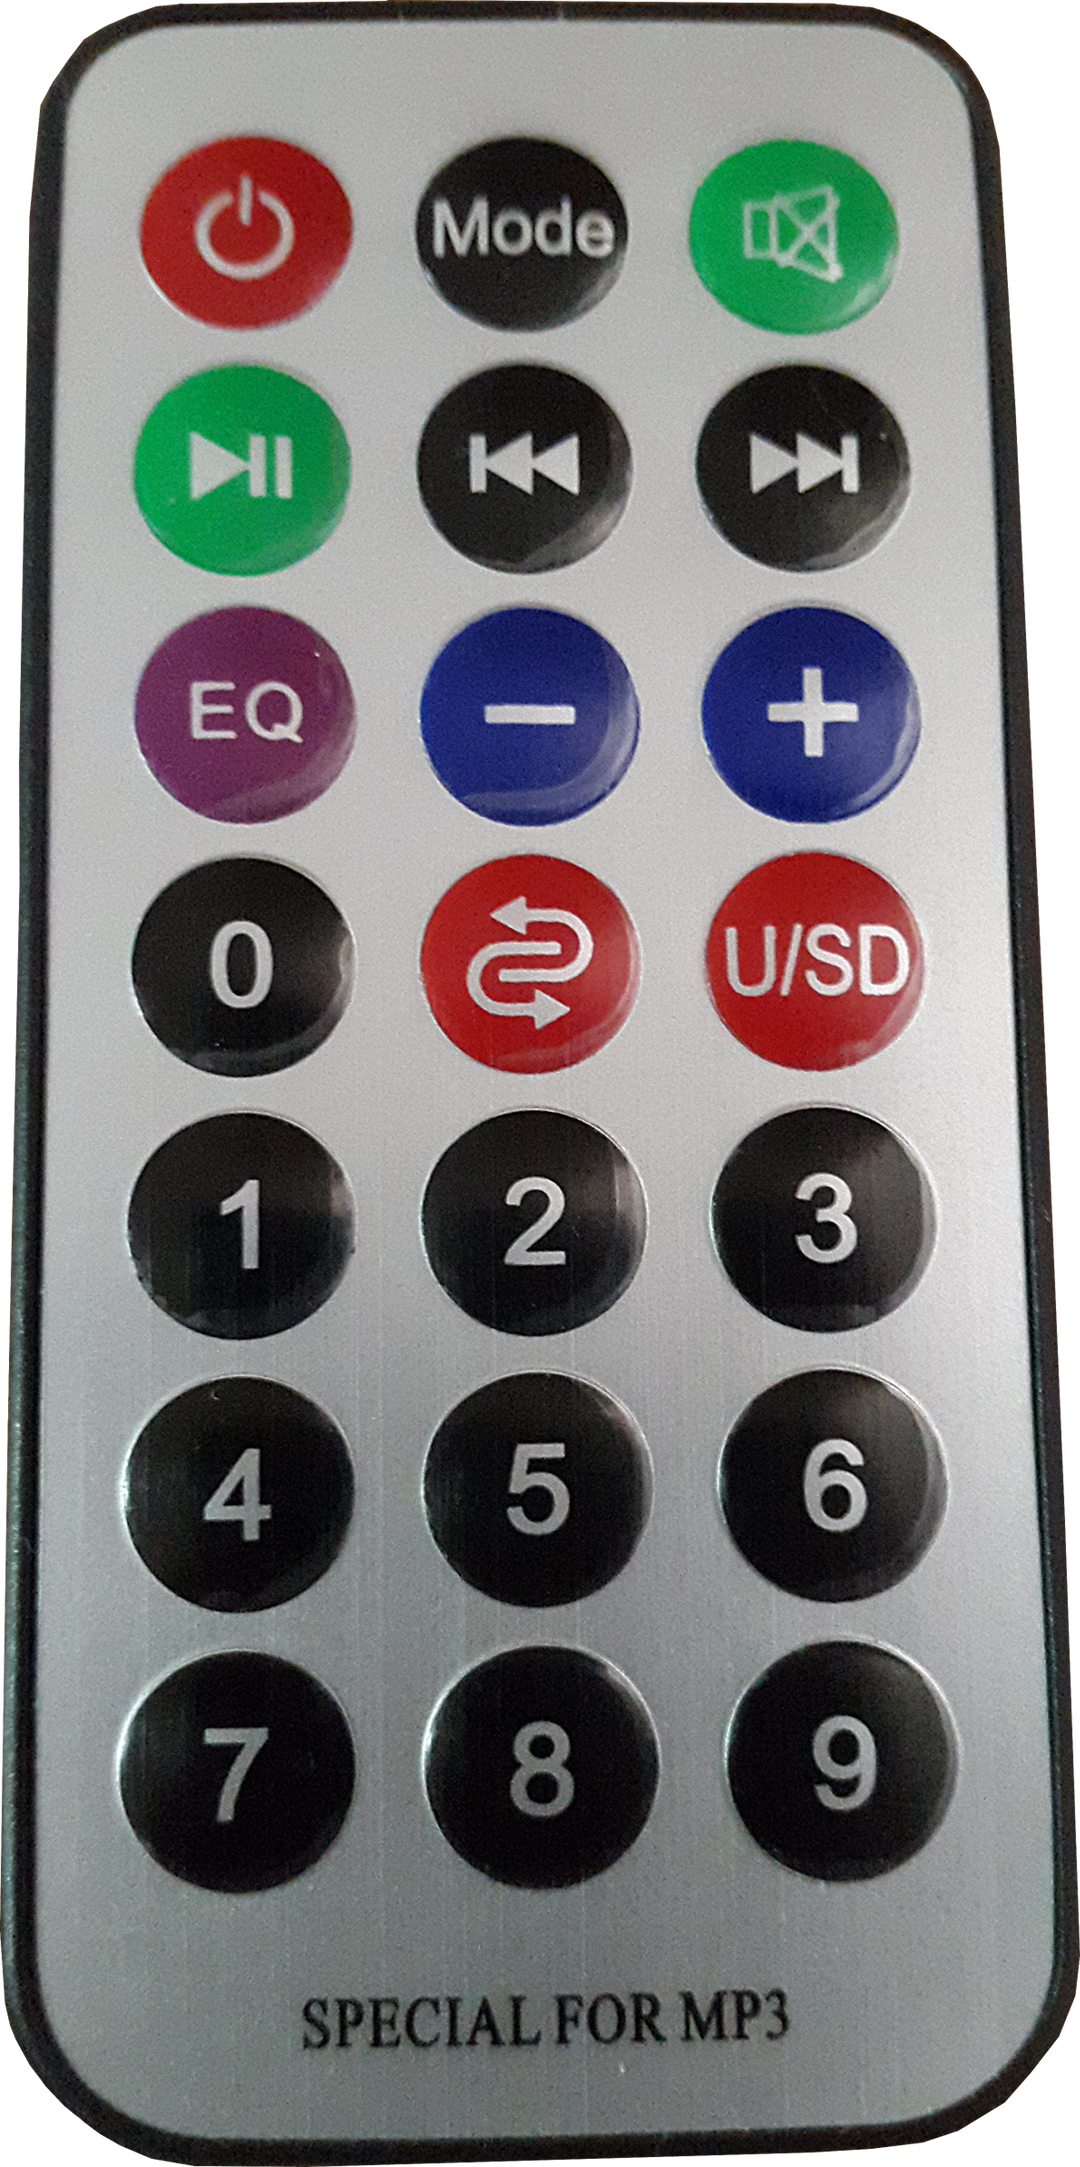
\includegraphics[width=7cm]{ir}
    \end{figure}

% \newpage
% \section{Referências}

% [1] Chapman, S.J. -- Electric Machinery Fundamentals, 4th Edition;

% [2] Fitzgerald, A. E. -- Máquinas Elétricas, 2da Edição;

\end{document}